% PuTTYXming.tex
\section{PuTTY and Xming on Windows} \label{sec:puttyxming}

The PuTTY program provides a X11/ssh connection to remote machines. Here
the machine's hostname is \dhl{pier15.local}, the port is 22.

XMing is a X11 ``server'' (meaning is backwards from data client/server sense) that
``serves'' the graphics from a remote programming doing all the heavy computing.

Grab Xming and install on a Win machine.

First some X11 magic:

\begingroup \fontsize{10pt}{10pt}
\selectfont
%%\begin{Verbatim} [commandchars=\\\{\}]
\begin{verbatim} 
the files /etc/X11
/etc/X11/xinit/xserverrc
~/.xinitrc
~/.xsession  -- start programs when the login is complete
~/.profile

ssh-keygen -t ed25519 -C "your_email@example.com"

\end{verbatim}
\endgroup
%% \end{Verbatim}



\verb=xmodmap -pke > ~/.Xmodmap # make a .Xmodmap to hack upon=

This varies with new modern keyboards, there is massive
confusion over what a key is called. 

xev program will show keycodes when a key changes state,
like shift down, then shift up etc...
When using the ``caps'' key:

\verb/keycode  37 = Control_L NoSymbol Control_L/

\begingroup \fontsize{10pt}{10pt}
\selectfont
%%\begin{Verbatim} [commandchars=\\\{\}]
\begin{verbatim} 


\end{verbatim}
\endgroup
%% \end{Verbatim}


Run XLaunch verify settings:

\vspace{-.15cm}
\begin{enumerate}\addtolength{\itemsep}{-0.5\baselineskip}
%\setcounter{enumi}{N}
   \item   multiple windows
   \item   start no client
   \item   clipboard checked
   \item   save configuration
\end{enumerate}


Configure PuTTY:

\vspace{-.15cm}
\begin{enumerate}\addtolength{\itemsep}{-0.5\baselineskip}
%\setcounter{enumi}{N}
   \item   Session:
\vspace{-.15cm}
\begin{enumerate}\addtolength{\itemsep}{-0.5\baselineskip}
%\setcounter{enumi}{N}
   \item   hostname:pier15.local  port 22
   \item   CTM\_X
   \item   check Only on clean exit
\end{enumerate}
   \item   Window
\vspace{-.15cm}
\begin{enumerate}\addtolength{\itemsep}{-0.5\baselineskip}
%\setcounter{enumi}{N}
   \item   120 50
   \item   scrollback 200
   \item   display scrollbar
   \item   Reset scrollback on display activity
   \item   push erased text into scrollback
\end{enumerate}
   \item   Connection -> Data
\vspace{-.15cm}
\begin{enumerate}\addtolength{\itemsep}{-0.5\baselineskip}
%\setcounter{enumi}{N}
   \item   login name 
   \item   Terminal-type string xterm
   \item   Terminal Speed 38400, 38400
\end{enumerate}
   \item   SSH->X11
\vspace{-.15cm}
\begin{enumerate}\addtolength{\itemsep}{-0.5\baselineskip}
%\setcounter{enumi}{N}
   \item   Enable X11 forwarding
   \item   localhost:0.0
   \item   MIT-Magic-Cookie-1
\end{enumerate}

\end{enumerate}


On the Windows pane, enter a new configuration for this machine.

\begin{figure}[h!]
\centering
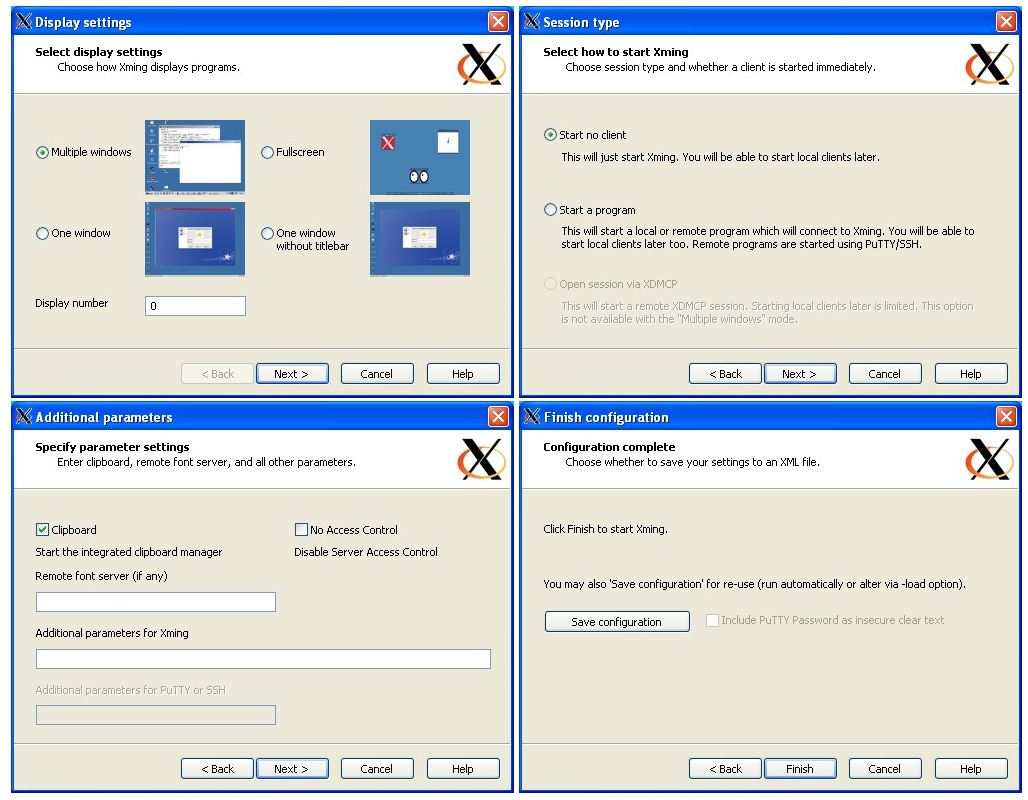
\includegraphics[width=.75\textwidth]{images/XmingConfig.png}
\caption{XMing screen snaps of the 4 configuration menu panels.} %% \caption{{\tiny{citation}}} 
\label{figure:}
\end{figure}

\begin{figure}[h!]
\centering
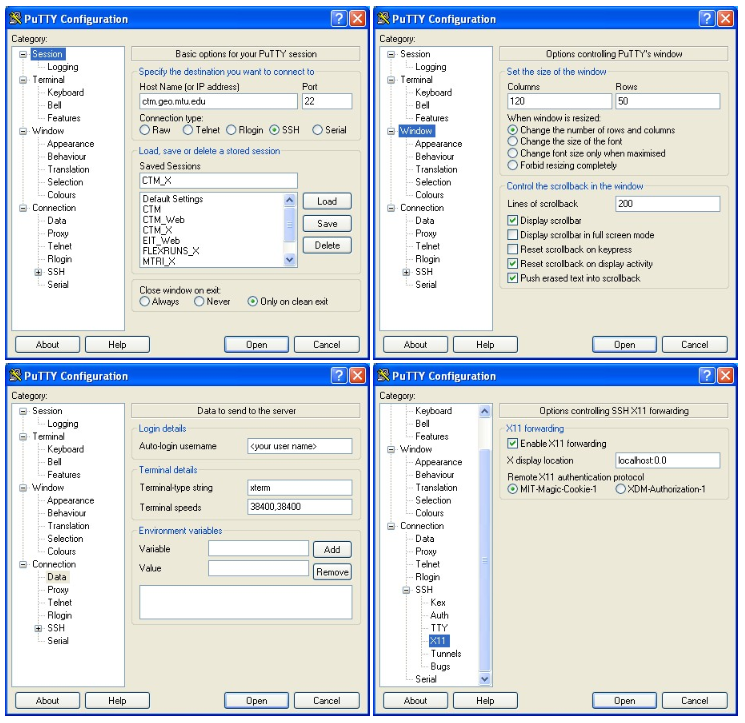
\includegraphics[width=.7\textwidth]{images/PuYYTXming.png}
\caption{PuTTY screen snaps of the 4 configuration menu panels.} %% \caption{{\tiny{citation}}} 
\label{figure:}
\end{figure}



